\section{Analisi e benchmark}

Per verificare che i metodi si comportassero in maniera corretta, abbiamo provato ad eseguire da interfaccia grafica una serie di test.



%%%%%%%%%%%%%%%%%%%%%%%%%%%%%%%%%%%%%%%%%%%%%%%%%%%%%%%%%%%%%%%%%%%%%%%%%%%%%%%%%%%%%%%%%%%%%%%%%%%%%%%%%%%%%%%%%%%%%%%%%%%%%%%%%%%%%%%%%%%%%%%%%%%%%%%%%%%%%%%%%%%%%%%%%%%%%%%%%%%%%%%%%%%%%%%%%%%%%%%%%%%%%%%%%%%%%%%%%%%%%%%%%%%%%%%%%%%%%%%%%%%%%%%%%%%%%%%%%%%%%%%%%%%%%%%%%%%%%%%

\subsection{Runtime data}

Le seguenti analisi nascono dai dati ricavati dall'esecuzione dei quattro metodi iterativi, i parametri considerati sono: \textit{tolleranza utilizzata} durante la fase di risoluzione, il \textit{tempo di esecuzione espresso in millisecondi}, il \textit{numero di iterazioni} effettuate per arrivare all'output, l'\textit{errore relativo} della soluzione ottenuta in relazione a quella di partenza e il \textit{nome della matrice risolta}. Il fine è quello di trarre delle conclusioni concrete sui quattro metodi iterativi, in particolare sulla loro funzionalità e performance.
(? e trarne una conclusione anche sui migliori parametri da inserire per ogni metodo?).


\subsubsection{Metodi iterativi a confronto}

\paragraph{tolerance/relativeError}
Abbiamo pensato di mettere in relazione l'errore relativo e la tolleranza utilizzata in fase di risoluzione dei quattro metodi a paragone, l'obiettivo è stabilire in che modo, al variare della tolleranza, il valore dell'errore relativo dei metodi potrebbe differire.

\paragraph{Difference between the methods}
%Immagine tolerance-relative_error, spa1, difference between the 4 methods
%Immagine tolerance-relative_error, spa2, difference between the 4 methods
%Immagine tolerance-relative_error, vem1, difference between the 4 methods
%Immagine tolerance-relative_error, vem2, difference between the 4 methods


\begin{figure}%
	\centering
	\subfloat{{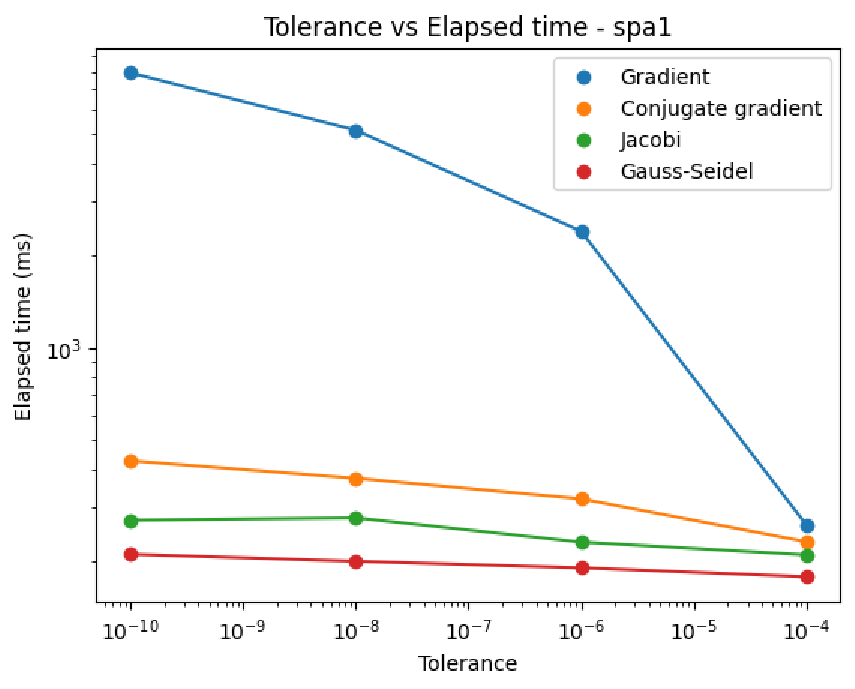
\includegraphics[width=0.40\textwidth]{figures/Tolerance vs Elapsed time/Difference between the 4 methods/spa1.pdf} }}%
	\subfloat{{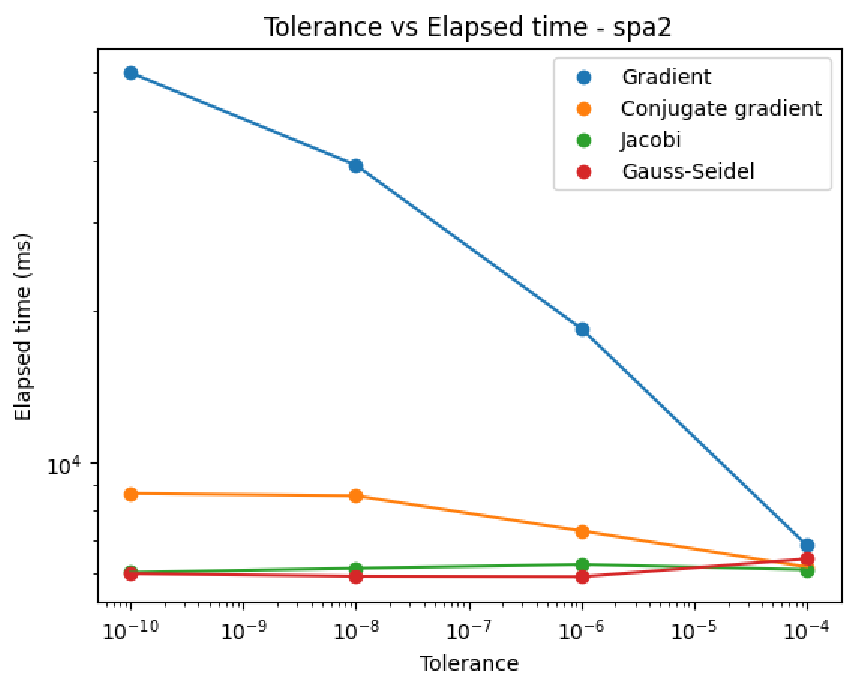
\includegraphics[width=0.40\textwidth]{figures/Tolerance vs Elapsed time/Difference between the 4 methods/spa2.pdf} }}%
	\qquad
	\subfloat{{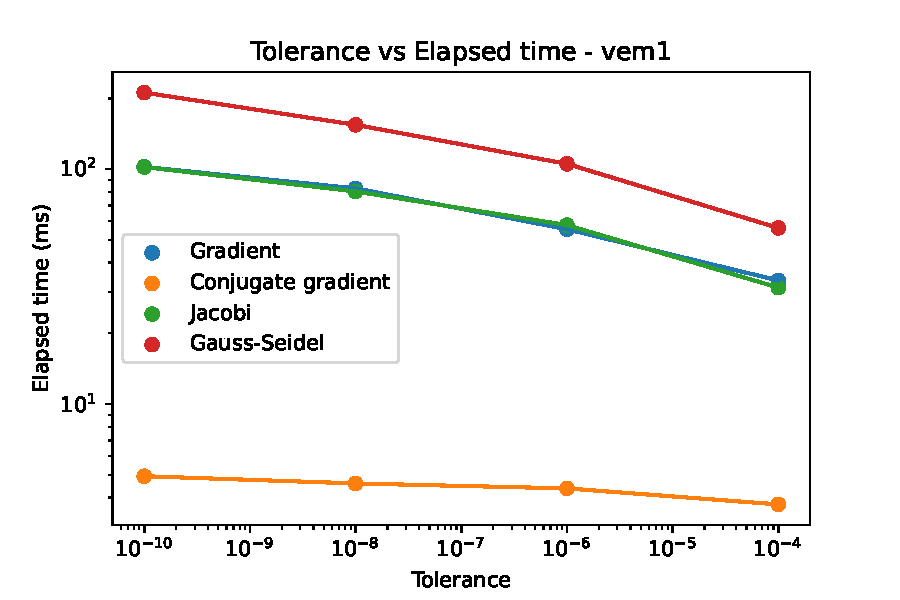
\includegraphics[width=0.40\textwidth]{figures/Tolerance vs Elapsed time/Difference between the 4 methods/vem1.pdf} }}%
	\subfloat{{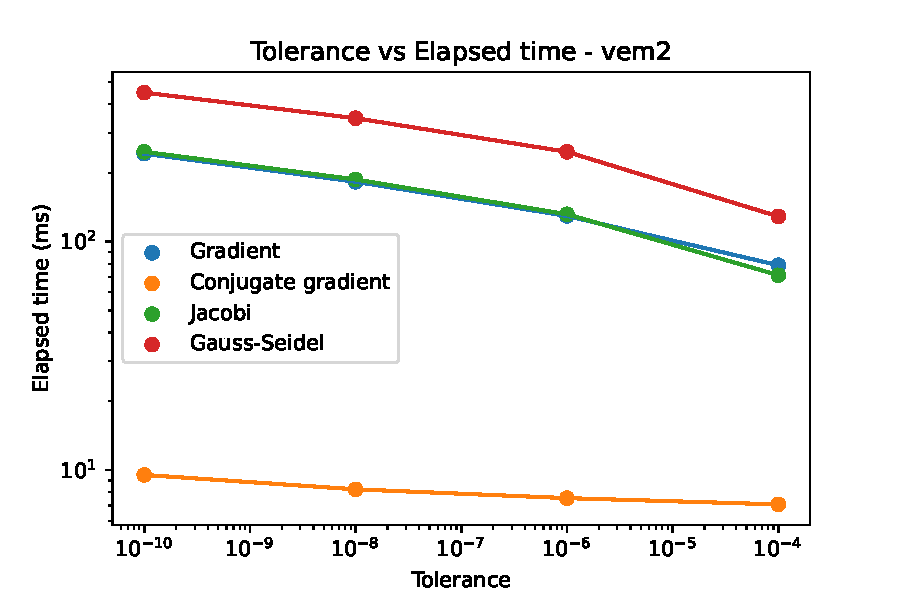
\includegraphics[width=0.40\textwidth]{figures/Tolerance vs Elapsed time/Difference between the 4 methods/vem2.pdf} }}%
	\caption{Grafici tolleranza / tempi sulle varie matrici di benchmark}%
\end{figure}

\begin{figure}%
	\centering
	\subfloat{{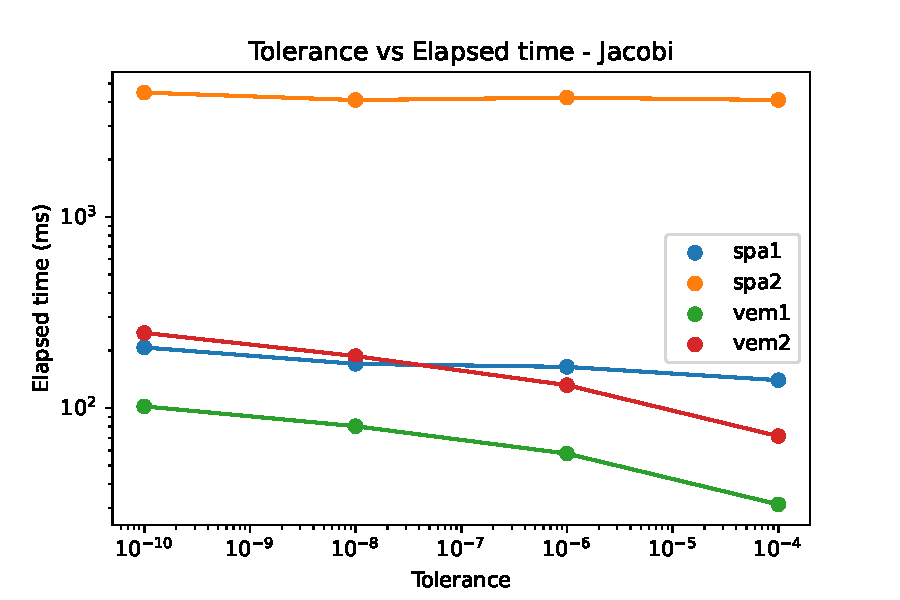
\includegraphics[width=0.40\textwidth]{figures/Tolerance vs Elapsed time/Difference between the 4 matrices on the same method/Jacobi.pdf} }}%
	\subfloat{{\includegraphics[width=0.40\textwidth]{figures/Tolerance vs Elapsed time/Difference between the 4 matrices on the same method/Conjugate Gradient.pdf} }}%
	\qquad
	\subfloat{{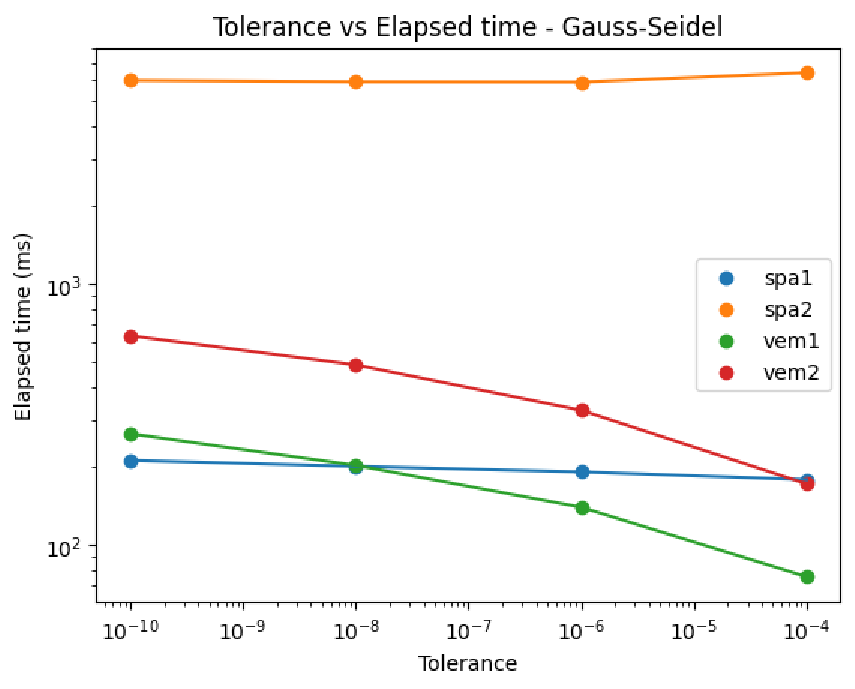
\includegraphics[width=0.40\textwidth]{figures/Tolerance vs Elapsed time/Difference between the 4 matrices on the same method/Gauss-Seidel.pdf} }}%
	\subfloat{{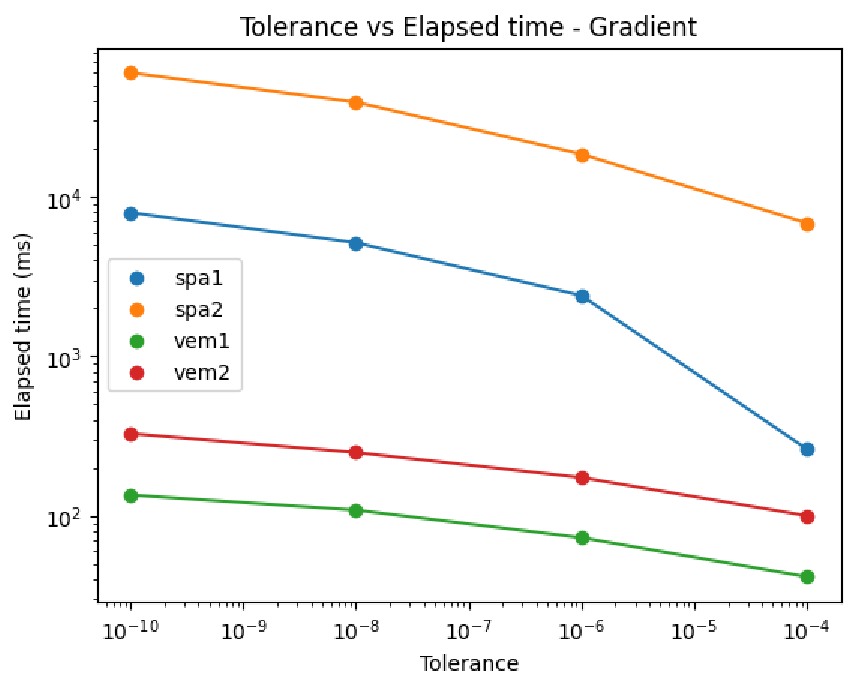
\includegraphics[width=0.40\textwidth]{figures/Tolerance vs Elapsed time/Difference between the 4 matrices on the same method/Gradient.pdf} }}%
	\caption{Grafici tolleranza / tempi rispetto i singoli metodi}%
\end{figure}



\paragraph{tolerance/elapsedTime}

%Immagine tolerance-elapsedTime, spa1, difference between the 4 methods
%Immagine tolerance-elapsedTime, spa2, difference between the 4 methods
%Immagine tolerance-elapsedTime, vem1, difference between the 4 methods
%Immagine tolerance-elapsedTime, vem2, difference between the 4 methods
Dai grafici, si evince immediatamente che all'aumentare della tolleranza, il tempo di esecuzione di ogni algoritmo cala, ed è più che ragionevole dato che al calare della tolleranza, il criterio di arresto diventa più permissivo.
Portando inevitabilmente, per tutti gli algoritmi, ad un numero inferiore di iterazione, conseguentemente ad un tempo di esecuzione minore ed una soluzione meno precisa.

\begin{figure}%
	\centering
	\subfloat{{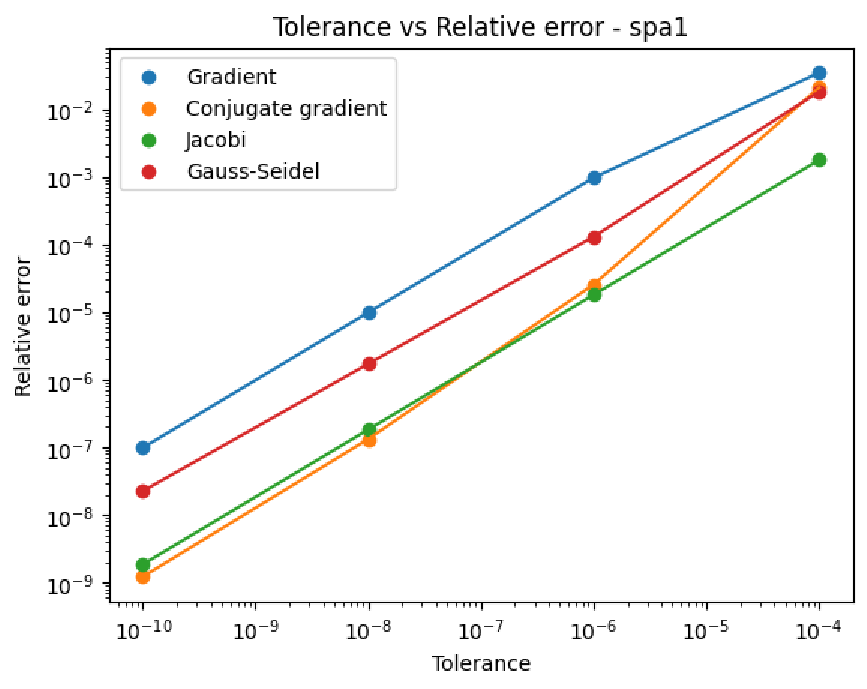
\includegraphics[width=0.40\textwidth]{figures/Tolerance vs Relative error/Difference between the 4 methods/spa1.pdf} }}%
	\subfloat{{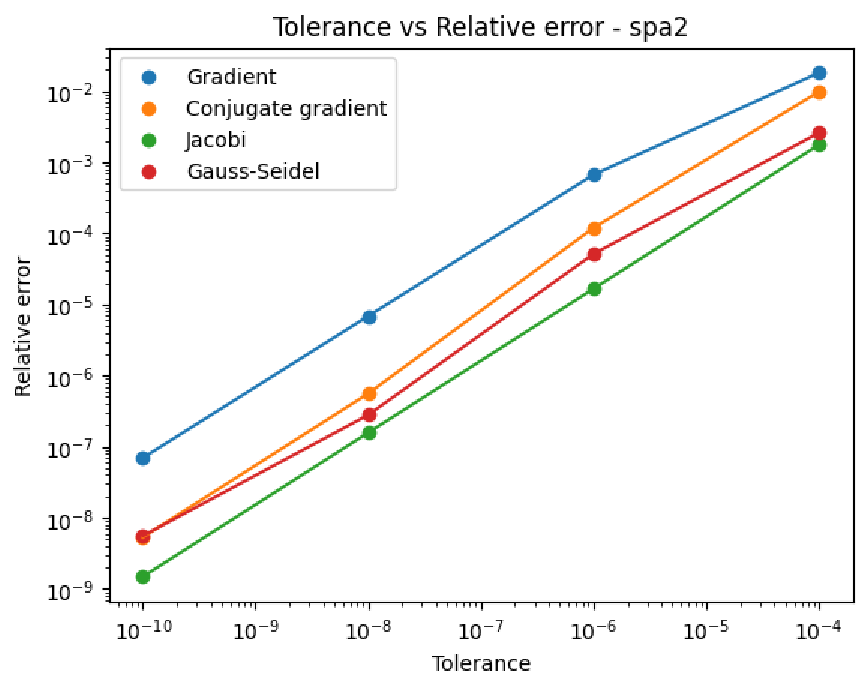
\includegraphics[width=0.40\textwidth]{figures/Tolerance vs Relative error/Difference between the 4 methods/spa2.pdf} }}%
	\qquad
	\subfloat{{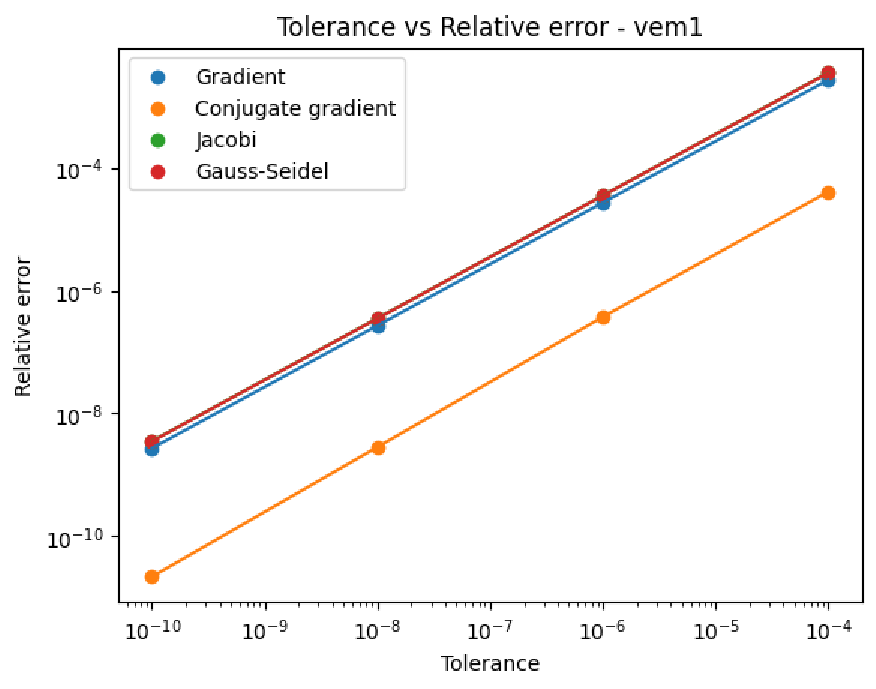
\includegraphics[width=0.40\textwidth]{figures/Tolerance vs Relative error/Difference between the 4 methods/vem1.pdf} }}%
	\subfloat{{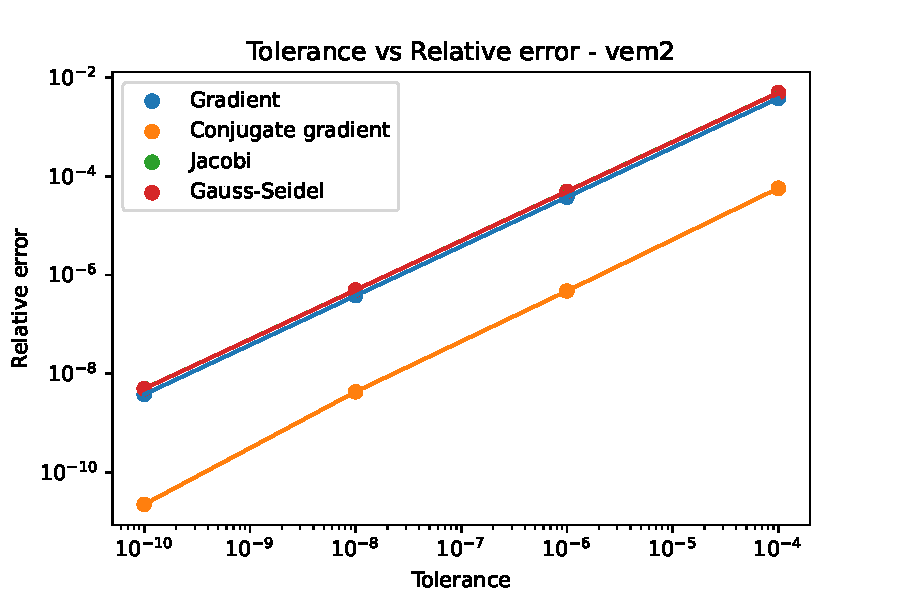
\includegraphics[width=0.40\textwidth]{figures/Tolerance vs Relative error/Difference between the 4 methods/vem2.pdf} }}%
	\caption{Grafici tolleranza / tempi sulle varie matrici di benchmark}%
\end{figure}


\begin{figure}%
	\centering
	\subfloat{{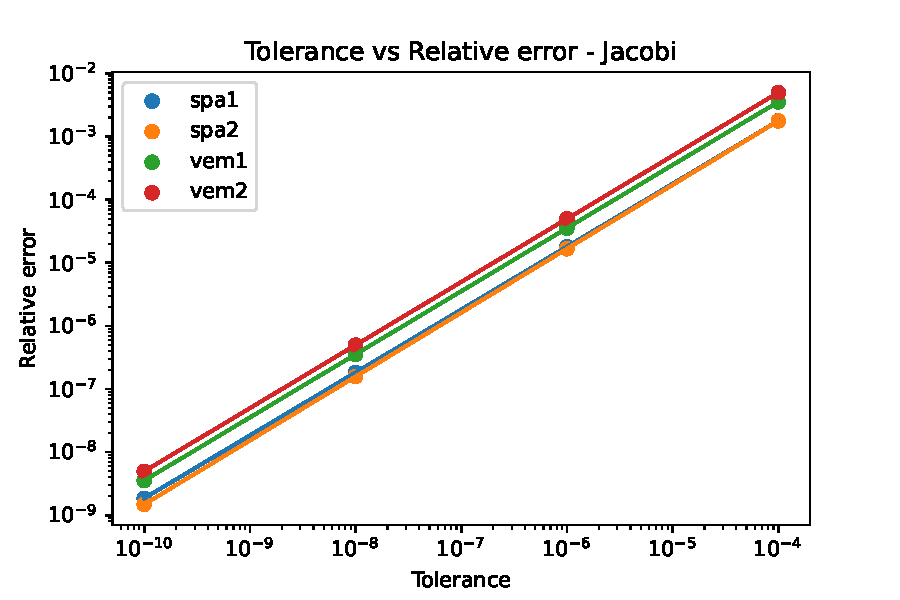
\includegraphics[width=0.40\textwidth]{figures/Tolerance vs Relative error/Difference between the 4 matrices on the same method/Jacobi.pdf} }}%
	\subfloat{{\includegraphics[width=0.40\textwidth]{figures/Tolerance vs Relative error/Difference between the 4 matrices on the same method/Conjugate Gradient.pdf} }}%
	\qquad
	\subfloat{{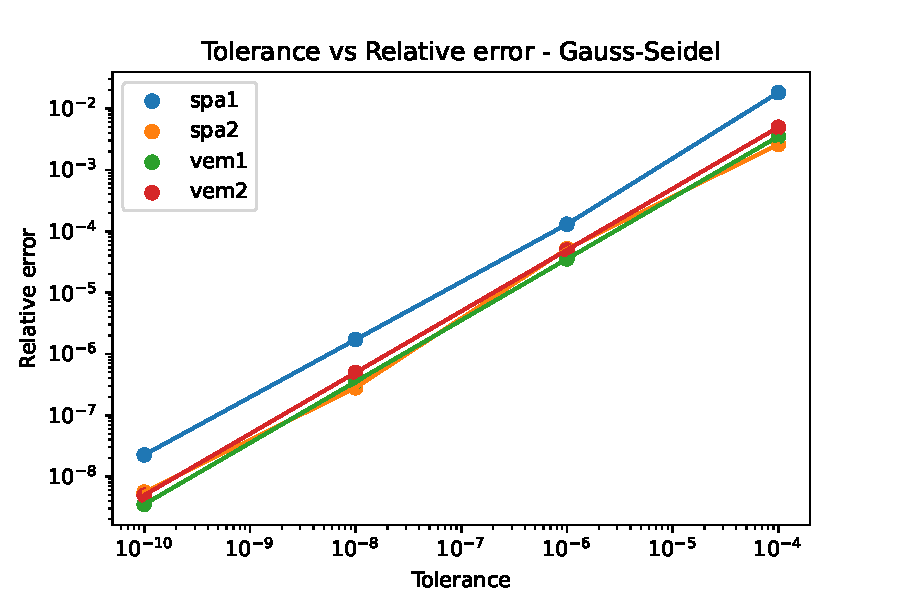
\includegraphics[width=0.40\textwidth]{figures/Tolerance vs Relative error/Difference between the 4 matrices on the same method/Gauss-Seidel.pdf} }}%
	\subfloat{{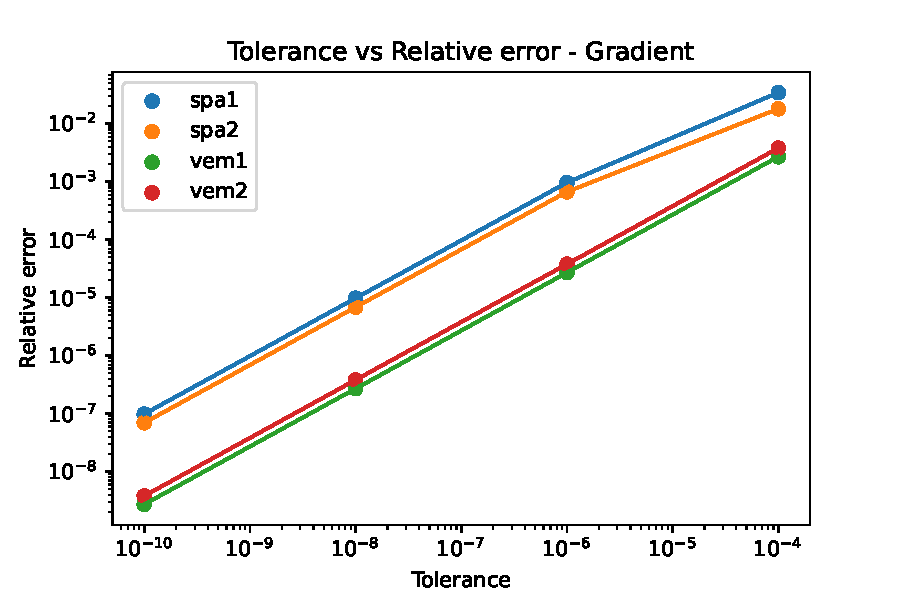
\includegraphics[width=0.40\textwidth]{figures/Tolerance vs Relative error/Difference between the 4 matrices on the same method/Gradient.pdf} }}%
	\caption{Grafici tolleranza / tempi rispetto i singoli metodi}%
\end{figure}


%%%%%%%%%%%%%%%%%%%%%%%%%%%%%%%%%%%%%%%%%%%%%%%%%%%%%%%%%%%%%%%%%%%%%%%%%%%%%%%%%%%%%%%%%%%%%
%%%%%%%%%%%%%%%%%%%%%%%%%%%%%%%%%%%%%%%%%%%%%%%%%%%%%%%%%%%%%%%%%%%%%%%%%%%%%%%%%%%%%%%%%%%%%
%%%%%%%%%%%%%%%%%%%%%%%%%%%%%%%%%%%%%%%%%%%%%%%%%%%%%%%%%%%%%%%%%%%%%%%%%%%%%%%%%%%%%%%%%%%%%

\subsubsection{Input a confronto}
Durante lo svolgimento dell'analisi, ci siamo resi conto che sarebbe stato interessante osservare la differenza della risoluzioni delle quattro matrici, al fine di stabilire in quali casi i metodi iterativi sono migliori con determinate strutture matriciali in input.

\paragraph{tolerance/relativeError}



